%
% File naaclhlt2013.tex
%

\documentclass[11pt,letterpaper]{article}
\usepackage{naaclhlt2013}
\usepackage{times}
\usepackage{graphicx}
\usepackage{latexsym}
\setlength\titlebox{6.5cm}    % Expanding the titlebox

\title{Large-scale Statistical Text Analytics in Relational Databases\Thanks{This
    document has been adapted from the instructions for earlier ACL
    and NAACL proceedings, including those for 
    NAACL-HLT-12 by Nizar Habash and William Schuler,
    NAACL-HLT-10 by Claudia Leacock and Richard Wicentowski,
    NAACL-HLT-09 by Joakim Nivre and Noah Smith, 
    for ACL-05 by Hwee Tou Ng and Kemal Oflazer,
    for ACL-02 by Eugene Charniak and Dekang Lin, and earlier ACL and
    EACL formats.  Those versions were written by several people,
    including John Chen, Henry S. Thompson and Donald Walker.
    Additional elements were taken from the formatting instructions of
    the {\em International Joint Conference on Artificial Intelligence}.  
    This second version clarifies the procedure for 
    submitting for double-blind reviewing.}}

\author{Kun Li\\
	    University of Florida\\
	    111 Anywhere Street\\
	    Mytown, NY 10000, USA\\
	    {\tt kli@cise.ufl.edu}
	  \And
	Christian Grant\\
  	University of Florida\\
  	900 Main Street\\
  	Ourcity, PQ, Canada A1A 1T2\\
  {\tt cgrant@cise.ufl.edu}}

\date{}

\begin{document}
\maketitle
\begin{abstract}
  This document contains the instructions for preparing a camera-ready
  manuscript for the proceedings of NAACL HLT 2013.  The document itself conforms
  to its own specifications, and is therefore an example of what
  your manuscript should look like.  Papers are required to conform to
  all the directions reported in this document.  Also included are instructions for
  submission to the conference, which are similar to the camera-ready instructions
  but remove author-identifying information.
\end{abstract}

\section{Introduction}
Conditional random field(CRF) is a type of discriminative undirected probabilistic graphical model.
Linear-chain CRFs are special CRFs which assume that the next state depends only on the current state. 
Linear-chain CRFs achieve start of art accuracy in some real world natural language processing tasks such
as part of speech tagging(POS) and named entity resolution(NER).

\section{In-database Implementation}

Manuscripts must be in two-column format.  Exceptions to the
two-column format include the title, as well as the 
authors' names and complete
addresses (only in the final version, not in the version submitted for review), 
which must be centered at the top of the first page (see
the guidelines in Subsection~\ref{ssec:first}), and any full-width
figures or tables.  Type single-spaced.  Do not number the pages.
Start all pages directly under the top margin.  See the guidelines
later regarding formatting the first page.

%% If the paper is produced by a printer, make sure that the quality
%% of the output is dark enough to photocopy well.  It may be necessary
%% to have your laser printer adjusted for this purpose.  Papers that are too
%% faint to reproduce well may not be included.

%% {\bf Do not print page numbers on the manuscript.}  Write them lightly
%% on the back of each page in the upper left corner along with the
%% (first) author's name.

The maximum length of a manuscript is eight (8) pages for the main
conference, printed single-sided, plus two (2) pages for references
(see Section~\ref{sec:length} for additional information on the
maximum number of pages).  Do not number the pages.

The review process is double-blind, so do not include any author information (names, addresses) when submitting a paper for review.  However, you should allocate space for the names and addresses so that they will fit in the final (accepted) version.  This is best done by either providing fake or blank names and addresses (as shown in this paper).
\subsection{System Architecture}
\begin{center}
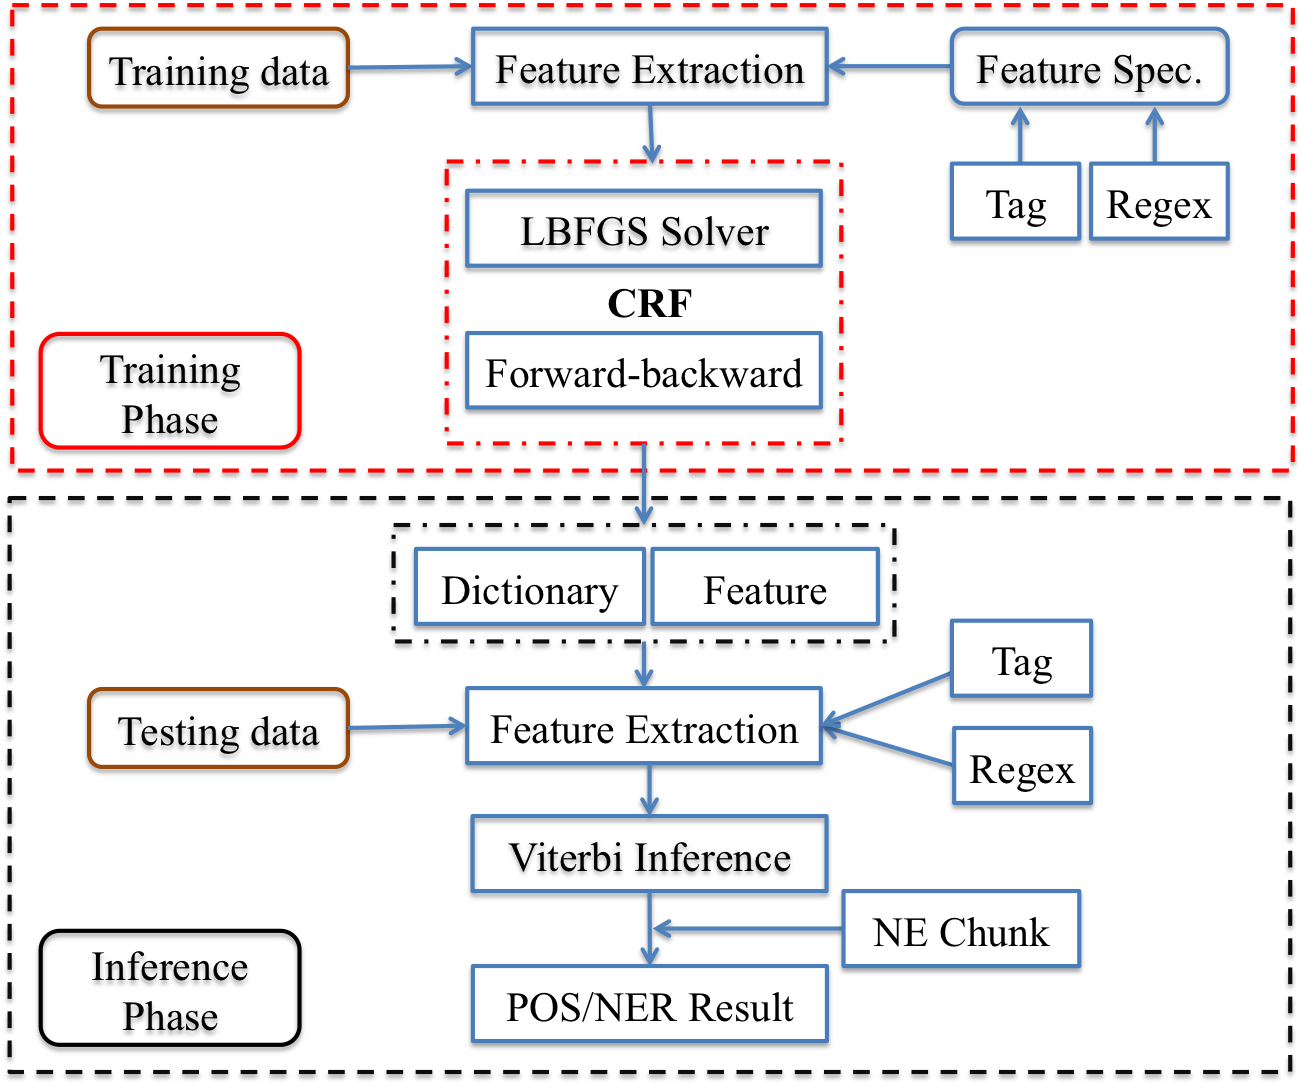
\includegraphics[height=15em]{system.png}
\end{center}

\subsection{Part-of-speech Tagging}
Part-of-speech tagging, also called grammatical tagging or word-category disambiguation is the process of assigning 
a part of speech to each word in a sentence. POS has been widely used in information retrieval and text to speech. 
There are two distinct methods for 
POS task: rule-based and stochastic.
In rule-based method, large collection of rules are defined to indentify the tag. Stochastic method is based on 
probabilistic graphic models such as hidden markov models and conditional random fields. In practice, 
conditional random fields are approved to achieve the state of art accuracy.

\subsubsection{Feature Extraction}
The Feature Extraction module provides functionality for basic text-analysis
tasks such as part-of-speech (POS) tagging and named-entity resolution.
At present, six feature types are implemented.
\begin{itemize}
\item Edge Feature: transition feature that encodes the transition feature weight from current label to next label.
\item Start Feature: fired when the current token is the first token in a sentence.
\item End Feature: fired when the current token is the last token in a sentence.
\item Word Feature: fired when the current token is observed in the trained dictionary.
\item Unknown Feature: fired when the current token is not observed in the trained dictionary for at least certain times.
\item Regex Feature: fired when the current token can be matched by the regular expression.
\end{itemize}

Advantages of extracting features using SQL statements:
\begin{itemize}
\item [$\star$] Decoupling the feature extraction and other code.
\item [$\star$] Compared with procedure language, SQL is much more easier to understand.
\item [$\star$] Storing all the features in tables avoids recomputing of features over iterations. It also boosts the performance.
\item [$\star$] SQL is naivelly paralleled.
\end{itemize}


\subsubsection{Parallel Linear-chain CRF Training}A Microsoft Word
\subsubsection{Parallel Linear-chain CRF Inference}
 The Viterbi algorithm is to find the top-k most likely labelings of a document 
for CRF models. 
We chose to implement a Python UDF that uses iterations to drive the Viterbi inference. 
In Greenplum, Viterbi can be run in parallel over different subsets 
of the document on a multi-core machine.

\subsection{Entity Detection}
\label{sect:pdf}


\begin{quote}
\begin{verbatim}
\usepackage{times}
\usepackage{latexsym}
\end{verbatim}
\end{quote}
in the preamble.

Additionally, it is of utmost importance to specify the {\bf
  US-Letter format} (8.5in $\times$ 11in) when formatting the paper.
When working with {\tt dvips}, for instance, one should specify {\tt
  -t letter}.

Print-outs of the PDF file on US-Letter paper should be identical to the
hardcopy version.  If you cannot meet the above requirements about the
production of your electronic submission, please contact the
publication chairs above  as soon as possible.


\subsection{Layout}
\label{ssec:layout}

Format manuscripts two columns to a page, in the manner these
instructions are formatted. The exact dimensions for a page on US-letter
paper are:

\begin{itemize}
\item Left and right margins: 1 inch
\item Top margin: 1 inch
\item Bottom margin: 1 inch
\item Column width: 3.15 inches
\item Column height: 9 inches
\item Gap between columns: 0.2 inches
\end{itemize}

\noindent Papers should not be submitted on any other paper size. Exceptionally,
authors for whom it is \emph{impossible} to format on US-Letter paper,
may format for \emph{A4} paper. In this case, they should keep the \emph{top}
and \emph{left} margins as given above, use the same column width,
height and gap, and modify the bottom and right margins as necessary.
Note that the text will no longer be centered.

\subsection{The First Page}
\label{ssec:first}

Center the title, author's name(s) and affiliation(s) across both
columns (or, in the case of initial submission, space for the names). 
Do not use footnotes for affiliations.  Do not include the
paper ID number assigned during the submission process. 
Use the two-column format only when you begin the abstract.

{\bf Title}: Place the title centered at the top of the first page, in
a 15 point bold font.  (For a complete guide to font sizes and styles, see Table~\ref{font-table}.)
Long title should be typed on two lines without
a blank line intervening. Approximately, put the title at 1in from the
top of the page, followed by a blank line, then the author's names(s),
and the affiliation on the following line.  Do not use only initials
for given names (middle initials are allowed). Do not format surnames
in all capitals (e.g., ``Bangalore,'' not ``BANGALORE'').  The affiliation should
contain the author's complete address, and if possible an electronic
mail address. Leave about 0.75in between the affiliation and the body
of the first page.

{\bf Abstract}: Type the abstract at the beginning of the first
column.  The width of the abstract text should be smaller than the
width of the columns for the text in the body of the paper by about
0.25in on each side.  Center the word {\bf Abstract} in a 12 point
bold font above the body of the abstract. The abstract should be a
concise summary of the general thesis and conclusions of the paper.
It should be no longer than 200 words.  The abstract text should be in 10 point font.

{\bf Text}: Begin typing the main body of the text immediately after
the abstract, observing the two-column format as shown in 
the present document.  Do not include page numbers.

{\bf Indent} when starting a new paragraph. For reasons of uniformity,
use Adobe's {\bf Times Roman} fonts, with 11 points for text and 
subsection headings, 12 points for section headings and 15 points for
the title.  If Times Roman is unavailable, use {\bf Computer Modern
  Roman} (\LaTeX2e{}'s default; see section \ref{sect:pdf} above).
Note that the latter is about 10\% less dense than Adobe's Times Roman
font.

\subsection{Sections}

{\bf Headings}: Type and label section and subsection headings in the
style shown on the present document.  Use numbered sections (Arabic
numerals) in order to facilitate cross references. Number subsections
with the section number and the subsection number separated by a dot,
in Arabic numerals. 

{\bf Citations}: Citations within the text appear
in parentheses as~\cite{Gusfield:97} or, if the author's name appears in
the text itself, as Gusfield~\shortcite{Gusfield:97}. In \LaTeX2e, the former is accomplished using
\verb|\cite| and the latter with \verb|\shortcite| or \verb|\newcite|.
Append lowercase letters to the year in cases of ambiguities.  
Treat double authors as in~\cite{Aho:72}, but write as 
in~\cite{Chandra:81} when more than two authors are involved. 
Collapse multiple citations as in~\cite{Gusfield:97,Aho:72}.

\textbf{References}: Gather the full set of references together under
the heading {\bf References}; place the section before any Appendices,
unless they contain references. Arrange the references alphabetically
by first author, rather than by order of occurrence in the text.
Provide as complete a citation as possible, using a consistent format,
such as the one for {\em Computational Linguistics\/} or the one in the 
{\em Publication Manual of the American 
Psychological Association\/}~\cite{APA:83}.  Use of full names for
authors rather than initials is preferred.  A list of abbreviations
for common computer science journals can be found in the ACM 
{\em Computing Reviews\/}~\cite{ACM:83}.

The \LaTeX{} and Bib\TeX{} style files provided roughly fit the
American Psychological Association format, allowing regular citations, 
short citations and multiple citations as described above.

{\bf Appendices}: Appendices, if any, directly follow the text and the
references (but see above).  Letter them in sequence and provide an
informative title: {\bf Appendix A. Title of Appendix}.

\textbf{Acknowledgment} sections should go as a last (unnumbered) section immediately
before the references.  

\subsection{Footnotes}

{\bf Footnotes}: Put footnotes at the bottom of the page. They may
be numbered or referred to by asterisks or other
symbols.\footnote{This is how a footnote should appear.} Footnotes
should be separated from the text by a line.\footnote{Note the
line separating the footnotes from the text.}  Footnotes should be in 9 point font.

\subsection{Graphics}

{\bf Illustrations}: Place figures, tables, and photographs in the
paper near where they are first discussed, rather than at the end, if
possible.  Wide illustrations may run across both columns and should be placed at
the top of a page. Color illustrations are discouraged, unless you have verified that 
they will be understandable when printed in black ink. 

\begin{table}
\begin{center}
\begin{tabular}{|l|rl|}
\hline \bf Type of Text & \bf Font Size & \bf Style \\ \hline
paper title & 15 pt & bold \\
author names & 12 pt & bold \\
author affiliation & 12 pt & \\
the word ``Abstract'' & 12 pt & bold \\
section titles & 12 pt & bold \\
document text & 11 pt  &\\
abstract text & 10 pt & \\
captions & 10 pt & \\
bibliography & 10 pt & \\
footnotes & 9 pt & \\
\hline
\end{tabular}
\end{center}
\caption{\label{font-table} Font guide. }
\end{table}

{\bf Captions}: Provide a caption for every illustration; number each one
sequentially in the form:  ``Figure 1. Caption of the Figure.'' ``Table 1.
Caption of the Table.''  Type the captions of the figures and 
tables below the body, using 10 point text.  

\subsection{Accessibility}
\label{ssec:accessibility}

In an effort to accommodate the color-blind (as well as those printing to paper), grayscale
readability for all accepted papers will be enforced.  Color is not forbidden, but authors should
ensure that tables and figures do not rely solely on color to convey critical distinctions.

\section{Performance Evaluation}
\label{sec:length}

\subsection{Scalability}
The NAACL HLT 2013 main conference accepts submissions of long papers
and short papers.  The maximum length of a long paper manuscript is
eight (8) pages of content and two (2) additional pages of references
\emph{only} (appendices count against the eight pages, not the
additional two pages).  The maximum length of a short paper manuscript
is four (4) pages and two (2) additional pages of references.  

\subsection{Comparisons with the State of Art}

For both long and short papers, all illustrations, references, and
appendices must be accommodated within these page limits, observing
the formatting instructions given in the present document.  Papers
that do not conform to the specified length and formatting
requirements are subject to be rejected without review.

\section{User Case: Tweet Analysis}
\label{sec:blind}

As the reviewing will be blind, the paper must not include the authors' names and affiliations. Furthermore, self-references that reveal the author's identity, e.g., ``We previously showed (Smith, 1991) ...'' must be avoided. Instead, use citations such as ``Smith previously showed (Smith, 1991) ...'' Papers that do not conform to these requirements will be rejected without review. In addition, please do not post your submissions on the web until after the review process is complete.

\section*{Acknowledgments}
Christan Grant is funded by a National
Science Foundation Graduate Research Fellowship under Grant No. DGE-0802270.
This work was supported by a gift from EMC Greenplum.

\begin{thebibliography}{}

\bibitem[\protect\citename{Aho and Ullman}1972]{Aho:72}
Alfred~V. Aho and Jeffrey~D. Ullman.
\newblock 1972.
\newblock {\em The Theory of Parsing, Translation and Compiling}, volume~1.
\newblock Prentice-{Hall}, Englewood Cliffs, NJ.

\bibitem[\protect\citename{{American Psychological Association}}1983]{APA:83}
{American Psychological Association}.
\newblock 1983.
\newblock {\em Publications Manual}.
\newblock American Psychological Association, Washington, DC.

\bibitem[\protect\citename{{Association for Computing Machinery}}1983]{ACM:83}
{Association for Computing Machinery}.
\newblock 1983.
\newblock {\em Computing Reviews}, 24(11):503--512.

\bibitem[\protect\citename{Chandra \bgroup et al.\egroup }1981]{Chandra:81}
Ashok~K. Chandra, Dexter~C. Kozen, and Larry~J. Stockmeyer.
\newblock 1981.
\newblock Alternation.
\newblock {\em Journal of the Association for Computing Machinery},
  28(1):114--133.

\bibitem[\protect\citename{Gusfield}1997]{Gusfield:97}
Dan Gusfield.
\newblock 1997.
\newblock {\em Algorithms on Strings, Trees and Sequences}.
\newblock Cambridge University Press, Cambridge, UK.

\end{thebibliography}

\end{document}
